\section{Methods}
\label{sec:methods}

Fig.~\ref{fig:pipeline} summarises the pipeline. The same preprocessing functions are called by the dataset builder, the training and evaluation code and the web service, so that training and serving cannot drift apart.

\begin{figure}[t]
\centering
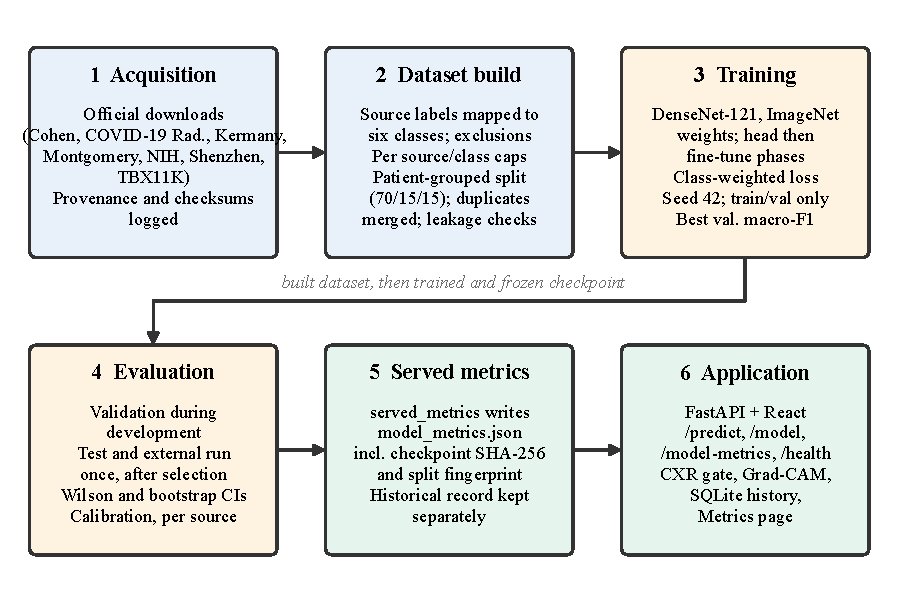
\includegraphics[width=\linewidth]{fig_pipeline.pdf}
\caption{End-to-end pipeline: acquisition with provenance, dataset build (labelling rules, caps, patient- and duplicate-grouped split, leakage checks), training with checkpoint selection on validation, once-only evaluation on the internal test split and the external cohort, and the metrics file served by the application.}
\label{fig:pipeline}
\end{figure}

\subsection{Preprocessing}
\label{sec:preproc}
Each image is decoded to an 8-bit, three-channel RGB array $I$ (grey-level images are replicated across channels and any alpha channel is dropped). Four deterministic steps follow, illustrated in Fig.~\ref{fig:preproc}.

\paragraph{Gaussian pre-blur} A $3\times3$ Gaussian kernel with $\sigma_1=0.8$ suppresses pixel-level noise and compression artefacts before contrast enhancement, which would otherwise amplify them:
\begin{equation}
I_1 = G_{\sigma_1} * I,\qquad
G_{\sigma}(x,y)=\frac{1}{Z_\sigma}\exp\!\left(-\frac{x^2+y^2}{2\sigma^2}\right),
\label{eq:blur}
\end{equation}
where $*$ denotes two-dimensional convolution applied per channel and $Z_\sigma$ normalises the discrete kernel to unit sum.

\paragraph{Contrast-limited adaptive histogram equalisation} $I_1$ is converted to the CIE $L^*a^*b^*$ colour space and CLAHE~\cite{pizer1987adaptive,zuiderveld1994contrast} is applied to the lightness channel $L$ only. The image is divided into an $8\times8$ grid of tiles. In tile $t$ with $M_t$ pixels and histogram $h_t(v)$ over $V=256$ grey levels, the histogram is clipped at
\begin{equation}
\beta_t = \max\!\left(1,\ \left\lfloor c\,\frac{M_t}{V}\right\rfloor\right),\qquad c=2.0,
\end{equation}
and the clipped excess $E_t=\sum_v \max(0,h_t(v)-\beta_t)$ is redistributed uniformly, $\tilde h_t(v)=\min(h_t(v),\beta_t)+E_t/V$. The tile mapping is the scaled cumulative distribution
\begin{equation}
T_t(v)=\frac{V-1}{M_t}\sum_{u=0}^{v}\tilde h_t(u),
\label{eq:clahe}
\end{equation}
and the output value of each pixel is the bilinear interpolation of the mappings of the four nearest tile centres, which avoids block artefacts. Clipping limits the slope of $T_t$ and therefore the amplification of noise in homogeneous regions. The enhanced $L$ channel is recombined with the unchanged $a^*,b^*$ channels and converted back to RGB, giving $I_2$.

\paragraph{Gaussian low-pass filter} A second Gaussian filter with $\sigma_2=1.0$ and kernel size $k=2\lceil 3\sigma_2\rceil+1=7$ is applied, $I_3=G_{\sigma_2}*I_2$. In the frequency domain the filter attenuates spatial frequency $(u,v)$ (in cycles per pixel) by
\begin{equation}
H(u,v)=\exp\!\left(-2\pi^2\sigma_2^2\,(u^2+v^2)\right),
\label{eq:lowpass}
\end{equation}
so that high-frequency texture enhanced by CLAHE, together with fine-grained acquisition artefacts, is damped. The value $\sigma_2=1.0$ was chosen in the earlier V5 work by comparing ten candidate filters (Gaussian $\sigma\in\{1,2,3\}$, ideal and Butterworth low-pass filters at three cut-offs each, and no filter) on the V5 validation split with a fixed baseline checkpoint and keeping the highest validation macro-F1. It was not re-tuned on V6; a run without the three filters is described in Section~\ref{sec:followup}.

\paragraph{Resizing and normalisation} $I_3$ is resized to $224\times224$ pixels with Lanczos interpolation (8$\times$8 support) and each channel $c$ is normalised with the ImageNet statistics,
\begin{equation}
x_c=\frac{I_{4,c}/255-\mu_c}{s_c},\qquad \boldsymbol\mu=(0.485,0.456,0.406),\ \ \mathbf{s}=(0.229,0.224,0.225).
\end{equation}
The three filters operate at the native resolution of each source image, before resizing. The same anatomy acquired at a different resolution therefore receives a different effective filter; this is a known limitation (Section~\ref{sec:limitations}). The builder caches the $224\times224$ result of the first four steps for each image, keyed by the SHA-256 of the raw file.

\begin{figure}[t]
\centering
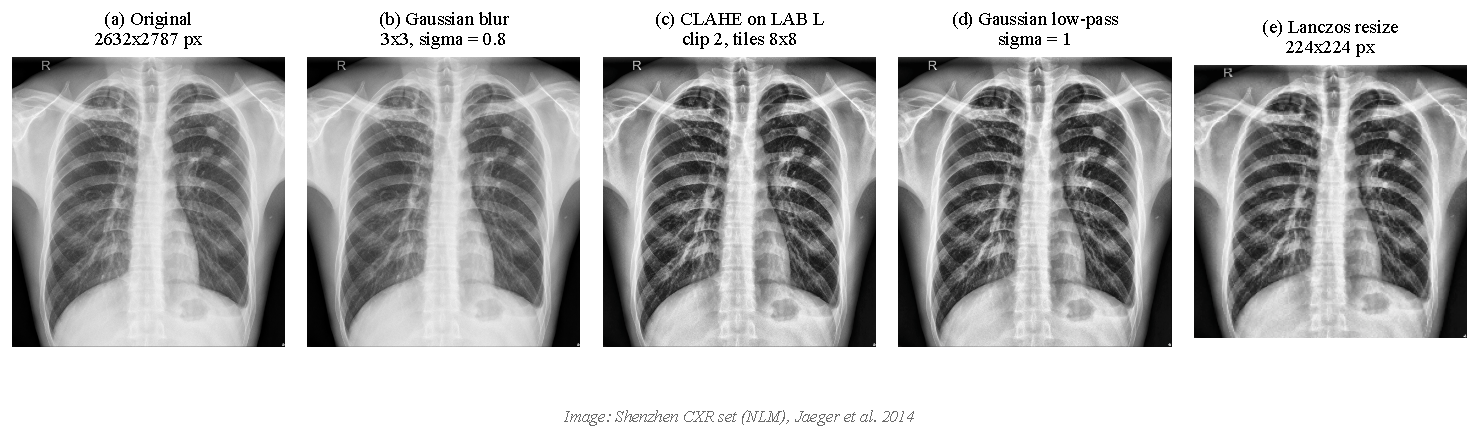
\includegraphics[width=\linewidth]{fig_preprocessing.pdf}
\caption{One radiograph through the preprocessing chain: input, Gaussian pre-blur ($\sigma_1=0.8$), CLAHE on the lightness channel (clip limit 2.0, $8\times8$ tiles), Gaussian low-pass ($\sigma_2=1.0$) and resizing to $224\times224$.}
\label{fig:preproc}
\end{figure}

\paragraph{Augmentation} During training only, each image is flipped horizontally with probability 0.5 and rotated by an angle drawn uniformly from $[-10^\circ,10^\circ]$ with reflected borders. Horizontal flipping reverses cardiac laterality; whether to keep it should be decided on validation in future work.

\subsection{Network}
The classifier (Fig.~\ref{fig:model}) is a DenseNet-121~\cite{huang2017densely} initialised with ImageNet weights~\cite{deng2009imagenet}, as in earlier chest radiograph work~\cite{rajpurkar2017chexnet}. Let $\phi(\mathbf{x})\in\mathbb{R}^{7\times7\times1024}$ be the final feature map of the backbone. The head computes
\begin{equation}
\mathbf{z}=\mathrm{GAP}(\phi(\mathbf{x})),\quad
\mathbf{a}=\mathrm{Dropout}_{0.3}\!\left(\mathrm{ReLU}\!\left(W_1\,\mathrm{BN}(\mathbf{z})+\mathbf{b}_1\right)\right),\quad
\mathbf{p}=\mathrm{softmax}(W_2\mathbf{a}+\mathbf{b}_2),
\label{eq:head}
\end{equation}
with global average pooling (GAP), batch normalisation (BN), $W_1\in\mathbb{R}^{256\times1024}$ and $W_2\in\mathbb{R}^{6\times256}$. The output $\mathbf{p}\in\Delta^5$ is the softmax score vector over the six classes, and the predicted class is $\hat y=\arg\max_k p_k$. The softmax scores are not calibrated probabilities of disease.

\begin{figure}[t]
\centering
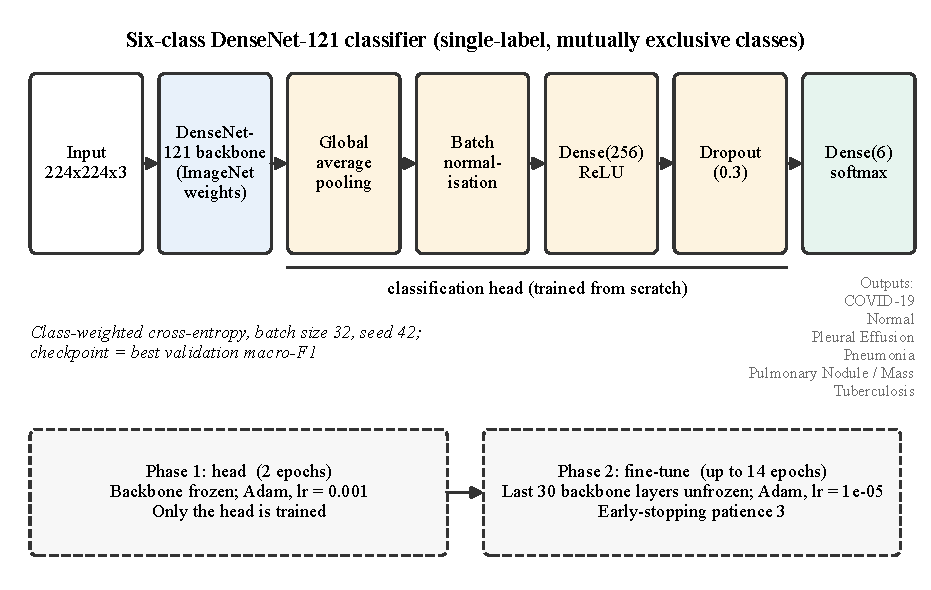
\includegraphics[width=\linewidth]{fig_model_architecture.pdf}
\caption{Model: DenseNet-121 backbone, global average pooling, batch normalisation, a 256-unit ReLU layer, dropout 0.3 and a six-way softmax. Phase~1 trains the head with the backbone frozen; phase~2 also unfreezes the last 30 backbone layers.}
\label{fig:model}
\end{figure}

\subsection{Loss with class weights}
The classes are imbalanced (Table~\ref{tab:builds}). With $n$ training images, $K=6$ classes and $n_k$ training images in class $k$, each training example receives the balanced weight
\begin{equation}
w_k=\frac{n}{K\,n_k},
\label{eq:weights}
\end{equation}
so that every class contributes the same total weight. The loss on a mini-batch $\mathcal{B}$ is the weighted categorical cross-entropy
\begin{equation}
\mathcal{L}(\theta)=\frac{1}{|\mathcal{B}|}\sum_{i\in\mathcal{B}} w_{y_i}\left(-\log p_{y_i}(\mathbf{x}_i;\theta)\right).
\label{eq:loss}
\end{equation}

\subsection{Two-phase optimisation}
Training uses Adam~\cite{kingma2015adam} with mini-batches of 32 and seed \RSeed{} for all random number generators. In phase~1 (two epochs) the backbone is frozen and only the head is trained with learning rate $10^{-3}$. In phase~2 the last 30 layers of the backbone are unfrozen and training continues with learning rate $10^{-5}$ until one of three conditions holds: three consecutive epochs without an improvement of validation macro-F1 (early stopping), the configured maximum number of phase-2 epochs, or a wall-clock budget. Batch-normalisation layers inside the unfrozen block are trained together with the convolutional layers. Each epoch is one pass over the training split.

\subsection{Checkpoint selection}
After every epoch the model is evaluated on the validation split and the checkpoint with the highest validation macro-F1 is kept, with validation macro ROC-AUC as tie-breaker:
\begin{equation}
e^\star=\arg\max_{e}\ \left(\mathrm{F1}^{\text{val}}_{\text{macro}}(e),\ \mathrm{AUC}^{\text{val}}_{\text{macro}}(e)\right)\quad\text{(lexicographic)}.
\end{equation}
Macro-F1 was chosen over accuracy because it weights the small COVID-19 and Tuberculosis classes equally with the large ones. Neither the internal test split nor the external cohort influences training or selection.

\subsection{Evaluation metrics}
\label{sec:metrics}
For class $k$ on a set of $N$ images, let $\mathrm{TP}_k$, $\mathrm{FP}_k$, $\mathrm{FN}_k$ and $\mathrm{TN}_k$ be the one-vs-rest counts derived from the $6\times6$ confusion matrix $C$ (rows true, columns predicted). Then
\begin{gather}
\mathrm{Prec}_k=\frac{\mathrm{TP}_k}{\mathrm{TP}_k+\mathrm{FP}_k},\quad
\mathrm{Rec}_k=\frac{\mathrm{TP}_k}{\mathrm{TP}_k+\mathrm{FN}_k},\quad
\mathrm{Spec}_k=\frac{\mathrm{TN}_k}{\mathrm{TN}_k+\mathrm{FP}_k},\quad
\mathrm{F1}_k=\frac{2\,\mathrm{Prec}_k\,\mathrm{Rec}_k}{\mathrm{Prec}_k+\mathrm{Rec}_k},\\
\mathrm{Acc}=\frac{1}{N}\sum_k C_{kk},\qquad
\mathrm{F1}_{\text{macro}}=\frac{1}{K}\sum_{k=1}^{K}\mathrm{F1}_k,\qquad
\mathrm{F1}_{\text{weighted}}=\sum_{k=1}^{K}\frac{N_k}{N}\,\mathrm{F1}_k ,
\end{gather}
where $N_k$ is the number of images of class $k$; macro precision and macro recall are defined analogously. A ratio with a zero denominator is reported as zero.

\paragraph{Ranking metrics} For class $k$, with positive set $P_k$ (images of class $k$) and negative set $Q_k$ (all others), the one-vs-rest ROC-AUC is the Mann--Whitney statistic on the score $p_k$,
\begin{equation}
\mathrm{AUC}_k=\frac{1}{|P_k||Q_k|}\sum_{i\in P_k}\sum_{j\in Q_k}\left(\mathbb{1}[p_{ik}>p_{jk}]+\tfrac12\,\mathbb{1}[p_{ik}=p_{jk}]\right),
\end{equation}
and macro ROC-AUC is the unweighted mean over the six classes. The precision--recall area (PR-AUC) is the average precision $\mathrm{AP}_k=\sum_n(R_n-R_{n-1})P_n$ over the thresholds $n$ of the ranked scores, with $P_n$ and $R_n$ the precision and recall at the $n$-th threshold; macro PR-AUC is the unweighted mean.

\paragraph{Calibration} The expected calibration error~\cite{naeini2015obtaining,guo2017calibration} is computed on the top-class score $\hat p_i=\max_k p_{ik}$ with $M=15$ equal-width bins $B_m$ on $[0,1]$:
\begin{equation}
\mathrm{ECE}=\sum_{m=1}^{M}\frac{|B_m|}{N}\left|\mathrm{acc}(B_m)-\mathrm{conf}(B_m)\right|,
\label{eq:ece}
\end{equation}
where $\mathrm{acc}(B_m)$ is the fraction of correct predictions and $\mathrm{conf}(B_m)$ the mean top-class score in bin $m$. No calibration map was fitted.

\paragraph{Confidence intervals} For a proportion $\hat\pi=x/n$ (accuracy, per-class recall, external sensitivity and specificity) we report the Wilson score interval~\cite{wilson1927probable} with $z=1.96$:
\begin{equation}
\frac{\hat\pi+\frac{z^2}{2n}\pm z\sqrt{\frac{\hat\pi(1-\hat\pi)}{n}+\frac{z^2}{4n^2}}}{1+\frac{z^2}{n}} .
\label{eq:wilson}
\end{equation}
For accuracy, macro-F1 and macro ROC-AUC we also compute a percentile bootstrap interval~\cite{efron1994introduction}: $B=2{,}000$ resamples of the $N$ test images drawn with replacement (seed 42), the metric $\hat\theta^{*}_b$ recomputed on each, and the interval $[\hat\theta^{*}_{(2.5)},\hat\theta^{*}_{(97.5)}]$ given by the 2.5th and 97.5th percentiles. For macro ROC-AUC only resamples that contain all six classes are used. These intervals describe sampling variation of the test set for a fixed model; they do not include variation due to training (seed, data order), which was not measured.

\subsection{External binary task}
\label{sec:exttask}
Montgomery contains only normal and TB radiographs, so the six-class metrics do not apply. We define a prediction as \emph{abnormal} if $\hat y\neq\text{Normal}$ and report
\begin{equation}
\mathrm{Sens}=\frac{\#\{\text{TB scans predicted abnormal}\}}{\#\{\text{TB scans}\}},\qquad
\mathrm{Spec}=\frac{\#\{\text{normal scans predicted Normal}\}}{\#\{\text{normal scans}\}},
\end{equation}
each with its Wilson interval, the exact Tuberculosis recall $\#\{\text{TB scans predicted Tuberculosis}\}/\#\{\text{TB scans}\}$, the ROC-AUC of the abnormality score $s=1-p_{\text{Normal}}$, and the full table of predicted classes for normal and TB scans. Sensitivity is never reported without specificity: a model that calls every image abnormal has a sensitivity of one. No threshold was tuned on the external cohort or on the internal test split.

\subsection{Grad-CAM}
Grad-CAM~\cite{selvaraju2017gradcam} maps are computed on the last ReLU activation of the backbone for the predicted class, upsampled to the input size and overlaid on the preprocessed image. They are used only for qualitative inspection; they show which regions influenced the class score, not radiological reasoning. Saliency methods including Grad-CAM have been found to fail localisation and sanity criteria on chest radiographs~\cite{arun2021assessing}, so we draw no conclusion from them about what the model has learned. The examples shown were selected by a rule fixed before any heatmap was viewed: for each class, the correctly classified test image whose top-class score is the median among the correctly classified test images of that class.
% Source of the rule: lungai/evaluation/make_figures.py::fig_gradcam_examples.

\subsection{Source-identifiability probe}
\label{sec:probe}
Per-source accuracy (Section~\ref{sec:res-source}) cannot separate a source effect from a difference in case mix. As a more direct control we asked whether the source collection of an image can be predicted from the features the classifier uses, both overall and among images of a single class. A classifier that recognises collections, as shown for hospital systems by Zech et~al.~\cite{zech2018variable}, could exploit any class--source association~\cite{degrave2021ai,geirhos2020shortcut}.

From build~2 we drew, separately for every (source, class) pair, at most 150 images of the training split and at most 100 images of the test split (fixed random seed), giving \RProbeNTrain{} probe-training and \RProbeNTest{} probe-test images; because the probe-training and probe-test images come from different splits, they are patient- and duplicate-separated as described in Section~\ref{sec:materials}. Each cached, preprocessed image (Section~\ref{sec:preproc}) was mapped to the 1024-dimensional GAP vector $\mathbf{z}$ of Eq.~\eqref{eq:head} by two frozen feature extractors: (i) DenseNet-121 with ImageNet weights only, which has learned nothing from this project, and (ii) the backbone of the selected model. Features were standardised with the mean and standard deviation of the probe-training set, and a multinomial logistic regression (L2 penalty with inverse strength $C=1$, class weights inversely proportional to source frequency) was fitted to predict the \emph{source}, not the disease. On the probe-test images we report the balanced accuracy, the mean over sources of the per-source recall, whose chance level is $1/S$ for $S$ sources; we report it over all images and within each class that has at least two sources in the probe-test set (Normal, Pneumonia, COVID-19 and Tuberculosis). Pleural Effusion and Nodule/Mass come from NIH only and cannot be probed within class. The probe does not influence any model or selection decision.
% Implementation: lungai/evaluation/source_probe.py (--per-group-train 150 --per-group-test 100 --seed 0); output artifacts/data_quality/source_probe_v6_build_002.json.

A high within-class balanced accuracy means that source information is linearly available in the features, so that a classifier \emph{could} separate classes by source style. It does not show that the trained classifier \emph{does} so; we therefore treat the probe as indirect evidence, to be read together with the per-source and external results.
